%%!TEX encoding = UTF-8 Unicode

% Several lines in file have comments suggesting common packages for the
% typical thesis in informatics or electronics developed at UA
% uncomment/comment the lines as required for your work
% Before each optional line you will have a small comment

% According to UA rules, font size should range from 10 to 12pt.
\documentclass[11pt,a4paper,oneside,onecolumn]{memoir}

\listfiles
%\fixpdflayout

\usepackage[utf8]{inputenc}

% Select Computer Modern Typewritter (For bold ttfamily in listings)
\usepackage{lmodern}
% OR... Bera Mono
%\usepackage[scaled]{beramono} % TTT Font
%\usepackage{anyfontsize} % As the name says...

\usepackage[T1]{fontenc}

% Enable for for Overleaf support
\usepackage{ifthen}
\def\useoverleaf{0}  % change to non-zero (for instance, 1) to enable it

\makeatletter
\newcommand{\makecoverfile}[0]{%
  \immediate\write18{latexmk -pdf cover.tex}%
}
\makeatother

% For PDF merging
\usepackage{pdfpages}
%\usepackage{setspace}


% Set DPI to 300
\pdfpxdimen=\dimexpr 1in/300\relax

% Allow the use of a larger number of packages
\usepackage{morewrites} 

% For English and Portuguese languages
% Portuguese will be the default.
% Uncomment \setlanguage below to change it
\usepackage[english,portuguese]{babel}

% Uncomment to use a custom date format
%\usepackage{datetime}
%\newdateformat{thesisdate}{\monthname[\THEMONTH] \THEYEAR} % Month Year

% Make pdf look better
\usepackage{microtype} 

% Uncomment to enable floats on facing pages
%\usepackage{dpfloat}

% Side by side figures
% Eg. Fig 1a, Fig 1b
\usepackage[hang,small,bf]{caption}
%\let\tion\undefined
%\let\subfloat\undefined
\usepackage{subcaption}

%\RequirePackage{textcase}

% Dropped Caps
%\usepackage{lettrine}

% Configure Hyperlink color
% As a matter or style, you may use this to enable/disable color boxes on links
%\usepackage[breaklinks=true,colorlinks=false,linkcolor=blue]{hyperref}
% Or use the default values provided by the hyperref package
\usepackage{hyperref}

% Redefine section names according to your preference
%\def\sectionautorefname{Section}
%\def\chapterautorefname{Chapter}
%\def\figureautorefname{Figure}
%\def\listingautorefname{Listing}
%\def\tableautorefname{Table}

% Redefine code boxes
%\ifthenelse{\equal{\useoverleaf}{0}}
%{\usepackage[outputdir=build]{minted}}
%{\usepackage{minted}}%

%\addto\captionsportuguese{%
%  \renewcommand\listingscaption{Código}
%}
%\fvset{fontsize=\footnotesize} % Make Code blocks smaller than text
%\usepackage{csquotes}

% Add support for PDF Comments
\usepackage{comment}
\ifthenelse{\equal{\useoverleaf}{0}}
{\usepackage{pdfcomment}}{}
\usepackage{bookmark} % New Bookmarks

% For Multiple columns in Glossary
\usepackage{multicol}

% Add support for Math symbols
\usepackage{amsmath}
\usepackage{amssymb}

% Add support for graphics
\usepackage{graphicx}
\graphicspath{{./figs/}}

% Add support for Colors
\usepackage{xcolor}

% Add support for the Euro symbol
\usepackage{eurosym}

% Add support for missingfigure and todo
\usepackage{todonotes}

% Setup bibliography with Biber using IEEE style for proper UTF-8 support
\usepackage[backend=biber, style=ieee, sorting=none, natbib=true, mincitenames=1, maxcitenames=2]{biblatex}
\bibliography{bib/references.bib}

% Use acronyms
\usepackage[printonlyused]{acronym} % For acronyms

% Indenting the first paragraph after section start
\usepackage{indentfirst}

% For fixing listoflistings with memoir
\usepackage{xparse}

% Uncomment the next lines to enable chart support through pgf and tikz
% This may require you to install further packages in your Tex system
%\usepackage[version=0.96]{pgf}
%\usepackage{tikz}

% UML support
%\usepackage{pgf-umlsd}

% Trees, Arrows, Mindmaps and other popular objects
%\usetikzlibrary{arrows,shadows,trees,shapes,decorations,automata,backgrounds,petri,mindmap} % for pgf-umlsd

% Package to master SI units
\usepackage[detect-weight=true, binary-units=true]{siunitx}
% For Electric Circuits
%\sisetup{load-configurations = binary}

% Set Voltage direction accordingly
% Option : oldvoltagedirection,nooldvoltagedirection,RPvoltages,EFvoltages
% More information at: https://mirrors.ibiblio.org/CTAN/graphics/pgf/contrib/circuitikz/doc/circuitikzmanual.pdf
% By default this template is using the Old Voltage Direction
%\usepackage[oldvoltagedirection,american,cuteinductors,smartlabels]{circuitikz}
%\usetikzlibrary{calc}
%\ctikzset{bipoles/thickness=1}
%\ctikzset{bipoles/length=0.8cm}
%\ctikzset{bipoles/diode/height=.375}
%\ctikzset{bipoles/diode/width=.3}
%\ctikzset{tripoles/thyristor/height=.8}
%\ctikzset{tripoles/thyristor/width=1}
%\ctikzset{bipoles/vsourceam/height/.initial=.7}
%\ctikzset{bipoles/vsourceam/width/.initial=.7}
%\tikzstyle{every node}=[font=\small]
%\tikzstyle{every path}=[line width=0.8pt,line cap=round,line join=round]

% For inline TT text (e.g. code snippets)
\usepackage{verbatim}

% Frames around figures and allow force placement
\usepackage{float}

% Configure Float style
%\floatstyle{boxed}
%\restylefloat{table}
%\restylefloat{figure}
%\restylefloat{lstlisting}

% For test purposes you may use the lipsum package to create dummy text
\usepackage{lipsum} % REMOVE

%Keep floats inside section!
\usepackage[section]{placeins}
\let \oldsubsubsection \subsubsection
\renewcommand{\subsubsection}[2][]{
  \FloatBarrier
  \oldsubsubsection#1{#2}
}
\let \oldsubsection \subsection
\renewcommand{\subsection}[2][]{
  \FloatBarrier
  \oldsubsection#1{#2}
}
\let \oldsection \section
\renewcommand{\section}[2][]{
  \FloatBarrier
  \oldsection#1{#2}
}
\let \oldchapter \chapter
\renewcommand{\chapter}[2][]{
  \FloatBarrier
  \oldchapter#1{#2}
}



% Use the built-in division styling
\headstyles{memman}

% Include subsections in the TOC
\settocdepth{subsection}

% Numbering down to subsections as well
\setsecnumdepth{subsection}

% extra index for first lines
\makeindex[lines]

% Margins for University of Aveiro Thesis
\setlrmarginsandblock{3cm}{2.5cm}{*}
\setulmarginsandblock{3cm}{3cm}{*}
\checkandfixthelayout

% Or select your custom spacing to make any ajustment
%\addtolength{\parskip}{0.5\baselineskip}
\linespread{1.5}

\newcommand\mainmatterWithoutReset
{\edef\temppagenumber{\arabic{page}}%
  \mainmatter
  \setcounter{page}{\temppagenumber}%
}


%%%%%%%%%%%%%%%%%%%%%%%%%%%%%%%%%%%%%%%%%%%%%%%%%%
% Document begins here
%%%%%%%%%%%%%%%%%%%%%%%%%%%%%%%%%%%%%%%%%%%%%%%%%%

\begin{document}

%Hi, I deleted the .aux and .toc .tof .lot .bbl and bcf and it seems working. - for next time

% Fix the numbering scheme by having a ghost style for page numbering
\pagenumbering{Alph}

\ifthenelse{\equal{\useoverleaf}{0}}{}{\makecoverfile{}}%
\setcounter{page}{0}
\includepdf[pages=-]{cover.pdf}

% Uncomment to enable English
\selectlanguage{english}


% Front matter

%Custom Chapter style named `thesis`
\makechapterstyle{thesis}{% Based on ell
  \chapterstyle{default}
  \renewcommand*{\chapnumfont}{\normalfont\sffamily}
  \renewcommand*{\chaptitlefont}{\normalfont\Huge\sffamily}
  \settowidth{\chapindent}{\chapnumfont 111}
  \renewcommand*{\chapterheadstart}{\begingroup
    \vspace*{\beforechapskip}%
    \begin{adjustwidth}{}{-\chapindent}%
    \hrulefill
    \smash{\rule{0.4pt}{15mm}}
    \end{adjustwidth}\endgroup}
  \renewcommand*{\printchaptername}{}
  \renewcommand*{\chapternamenum}{}
  \renewcommand*{\printchapternum}{%
    \begin{adjustwidth}{}{-\chapindent}
    \hfill
    \raisebox{10mm}[0pt][0pt]{\fontsize{30}{25}\selectfont\chapnumfont \thechapter}%
                              \hspace*{1em}
    \end{adjustwidth}\vspace*{-3.0\onelineskip}}
  \renewcommand*{\printchaptertitle}[1]{%
    \vskip\onelineskip
    \raggedleft {\chaptitlefont ##1}\par\nobreak\vskip 4\onelineskip}}


% Select chapter style from existing or select custom
%\chapterstyle{thesis} % Others: dowding, demo2, dash, chappell, brotherton, bianchi, ger, madsen, tatcher, veelo,indexes)
% thesis can also be used as defined previously
% Check the memoir documentation for the available themes
% Default is veelo
\chapterstyle{veelo}
\makeoddfoot{plain}{}{\thepage}{} % Added by André Zúquete to fix a page numbering issue on the veelo chapter style


% If you feel adventurous you can also define all aspects of your theme
% Use either this input or the chapterstyle before
% % Rules
\newcommand{\thinRule}{\rule{\textwidth}{0.25pt}}

% Customize heading appearances
% Define styles
\newcommand{\partSize}{\Huge}
\newcommand{\partStyle}{\lsstyle\scshape}
\newcommand{\chapterSize}{\Huge}
\newcommand{\chapterStyle}{\lsstyle\scshape}
\newcommand{\chapterAfter}{}
\newcommand{\sectionSize}{\Large}
\newcommand{\sectionStyle}{\scshape\MakeTextLowercase}
\newcommand{\subsectionSize}{\large}
\newcommand{\subsectionStyle}{\scshape\MakeTextLowercase}
\newcommand{\subsubsectionSize}{\large}
\newcommand{\subsubsectionStyle}{\scshape\MakeTextLowercase}
\newlength{\partNumSizePt}
\setlength{\partNumSizePt}{60pt}
\newlength{\chapterNumSizePt}
\setlength{\chapterNumSizePt}{60pt}
\newcommand{\partNumSize}{%
  \fontsize{\partNumSizePt}{1.2\partNumSizePt}\selectfont%
}
\newcommand{\partNumStyle}{\partChapterNumColor}
\newcommand{\chapterNumSize}{%
  \fontsize{\chapterNumSizePt}{1.2\chapterNumSizePt}\selectfont%
}
\newcommand{\chapterNumStyle}{\partChapterNumColor}

% Customize parts
\renewcommand{\partnamefont}{\partSize\partStyle}
\renewcommand{\partnumfont}{\partNumSize\partNumStyle}
\renewcommand{\printpartname}{}
\renewcommand{\printparttitle}[1]{%
  \normalfont\normalcolor\partnamefont #1
}

% Customize chapters
\makeatletter
\setlength{\beforechapskip}{30pt}
\renewcommand*{\chapterheadstart}{\vspace*{\beforechapskip}}
\setlength{\afterchapskip}{3ex}
\setlength{\midchapskip}{3ex}
\renewcommand*{\chapnamefont}{%
  \Large\flushright\chapterStyle\partChapterNumColor%
}
\renewcommand*{\chapnumfont}{\chapterNumSize\chapterNumStyle}
\renewcommand*{\chaptitlefont}{%
  \normalfont\flushleft\normalcolor\chapterSize\chapterStyle%
}
\renewcommand*{\printchaptername}{%
  \chapnamefont\MakeTextLowercase{\@chapapp}%
}
\renewcommand*{\chapternamenum}{\quad}
\renewcommand*{\printchapternum}{%
%  \chapnumfont\textls[-75]{\classicstylenums{\thechapter}}%
 \chapnumfont\textls[-75]{\thechapter}%

}
\renewcommand*{\printchaptertitle}[1]{%
  \chaptitlefont #1
  \chapterAfter
}
\makeatother
% Customize sections and subsections
\setsecnumformat{\csname my#1\endcsname\quad}
\setsecheadstyle{\sectionSize\sectionStyle}
\newcommand{\mysection}{{\thesection}}
\setlength{\beforesecskip}{3em}


\setsubsecheadstyle{\subsectionSize\subsectionStyle}
\newcommand{\mysubsection}{{\normalfont\subsectionSize\thesubsection}}
\setlength{\beforesubsecskip}{3em}

\setsubsubsecheadstyle{\subsubsectionSize\subsubsectionStyle}
\newcommand{\mysubsubsection}{{\normalfont\subsubsectionSize\thesubsubsection}}
\setlength{\beforesubsubsecskip}{2em}

% Customize "Table of ..." appearance
% Customize headings
\newcommand{\renewPrintXTitle}[1]{%
  \renewcommand{#1}[1]{%
    \printchaptertitle{##1}%
  }%
}
\renewPrintXTitle{\printtoctitle}
\renewPrintXTitle{\printlottitle}
\renewPrintXTitle{\printloftitle}

% Customize ToC headings
\renewcommand{\cftpartfont}{\partChapterNumColor\partStyle}
\renewcommand{\cftchapterfont}{\chapterStyle}
\renewcommand{\cftsectionfont}{}
\renewcommand{\cftsubsectionfont}{}
\renewcommand{\cftfigurefont}{}
\renewcommand{\cfttablefont}{}
\newcommand{\cftlstlistingfont}{}

% Increase number width
\newlength{\cftNumWidthIncrease}
\setlength{\cftNumWidthIncrease}{0.25em}
\addtolength{\cftpartnumwidth}{\cftNumWidthIncrease}
\addtolength{\cftchapternumwidth}{\cftNumWidthIncrease}
\addtolength{\cftsectionindent}{\cftNumWidthIncrease}
\addtolength{\cftsubsectionindent}{\cftNumWidthIncrease}
% No leader dots
%\renewcommand*{\cftpartdotsep}{\cftnodots}
%\renewcommand*{\cftchapterdotsep}{\cftnodots}
%\renewcommand*{\cftsectiondotsep}{\cftnodots}
%\renewcommand*{\cftsubsectiondotsep}{\cftnodots}
%\renewcommand*{\cftfiguredotsep}{\cftnodots}
%\renewcommand*{\cfttabledotsep}{\cftnodots}
%\newcommand*{\cftlstlistingdotsep}{\cftnodots}
% Set page numbers immediately after entry text
\newcommand{\tocEntryPageSep}{\hspace{1em}}
\renewcommand{\cftpartleader}{\cftdotfill{\cftdotsep}}
%\renewcommand{\cftpartafterpnum}{\cftparfillskip}
%\renewcommand{\cftchapterleader}{\tocEntryPageSep}
\renewcommand{\cftchapterleader}{\cftdotfill{\cftdotsep}}
%\renewcommand{\cftchapterafterpnum}{\cftparfillskip}
\renewcommand{\cftsectionleader}{\cftdotfill{\cftdotsep}}
%\renewcommand{\cftsectionafterpnum}{\cftparfillskip}
\renewcommand{\cftsubsectionleader}{\cftdotfill{\cftdotsep}}
%\renewcommand{\cftsubsectionafterpnum}{\cftparfillskip}
\renewcommand{\cftfigureleader}{\cftdotfill{\cftdotsep}}
%\renewcommand{\cftfigureafterpnum}{\cftparfillskip}
\renewcommand{\cfttableleader}{\cftdotfill{\cftdotsep}}
%\renewcommand{\cfttableafterpnum}{\cftparfillskip}
\newcommand{\cftlstlistingleader}{\cftdotfill{\cftdotsep}}
%\newcommand{\cftlstlistingafterpnum}{\cftparfillskip}
% Customize page numbers
\newcommand{\tocPageStyle}{\tocPageColor}
\renewcommand{\cftpartpagefont}{\tocPageStyle}
\renewcommand{\cftchapterpagefont}{\tocPageStyle}
\renewcommand{\cftsectionpagefont}{\tocPageStyle}
\renewcommand{\cftsubsectionpagefont}{\tocPageStyle}
\renewcommand{\cftfigurepagefont}{\tocPageStyle}
\renewcommand{\cfttablepagefont}{\tocPageStyle}
\newcommand{\cftlstlistingpagefont}{\tocPageStyle}

% Abstract
% Remove indents around abstract text
\setlength{\absleftindent}{0pt}
\setlength{\absrightindent}{0pt}
% Change font size to conform with the rest of the document text
\renewcommand{\abstracttextfont}{\normalsize}

% Customize headers and footers including page numbers
\newcommand{\hfTextSize}{\footnotesize}
\newcommand{\headTextStyle}{\lsstyle\scshape\MakeTextLowercase}
\nouppercaseheads
\makeevenhead{headings}%
             {\hfTextSize\thepage}%
             {}%
             {\hfTextSize\headTextStyle\leftmark}
\makeevenhead{plain}%
             {\hfTextSize\thepage}%
             {}%
             {\hfTextSize\headTextStyle\leftmark}
\makeoddhead{headings}%
            {\hfTextSize\headTextStyle\rightmark}%
            {}%
            {\hfTextSize\thepage}
\makeoddhead{plain}%
            {\hfTextSize\headTextStyle\rightmark}%
            {}%
            {\hfTextSize\thepage}


% Customize captions
\newcommand{\captionSize}{\small}
\newcommand{\captionStyle}{\scshape}
\newcommand{\captionWidthRatio}{0.9}

\captionnamefont{\captionSize\captionStyle}
\captiontitlefont{\captionSize}
\captiondelim{ -- }
\captiontitlefinal{}
\changecaptionwidth
%\captionwidth{\captionWidthRatio\textwidth}

% Define colors
%\newcommand{\titleColor}{\color[rgb]{0.616, 0.0627, 0.176}}
\newcommand{\titleColor}{\color[rgb]{0,0,0}}

\newcommand{\partChapterNumColor}{\titleColor}
\newcommand{\dropCapColor}{\titleColor}
%\newcommand{\tocPageColor}{\color[rgb]{0.0980, 0.329, 0.651}}

\newcommand{\tocPageColor}{\color[rgb]{0, 0,0}}
\definecolor{shade0}{rgb}{1.0 , 1.0 , 1.0 }
\definecolor{shade1}{rgb}{0.9 , 0.9 , 0.9 }
\definecolor{shade2}{rgb}{0.8 , 0.8 , 0.8 }
\definecolor{shade3}{rgb}{0.65, 0.65, 0.65}
\definecolor{shade4}{rgb}{0.45, 0.45, 0.45}
\definecolor{shade5}{rgb}{0.0 , 0.0 , 0.0 }



%Exclude sub figures from List of Figures
%\captionsetup[subfloat]{list=no}

% Texts
\newenvironment{introduction}
{%
  \begin{minipage}{\textwidth}%
   \itshape%
}
{%
  \end{minipage}%
  \par\addvspace{2\baselineskip plus 0.2\baselineskip minus 0.2\baselineskip}%
}

% Select Page style
\pagestyle{plain}

\frontmatter

\tightlists
\midsloppy
\raggedbottom

\setcounter{tocdepth}{2} %subsections are added to the TOC
\setcounter{secnumdepth}{4} %subsubsections are numbered

% Initial document tables start here: TOC, LOF, LOT, Glossary
% Table of contents with slightly smaller font
\cleardoublepage
{\small\tableofcontents}

% List of figures with slightly smaller font
\cleardoublepage
{\small\listoffigures}

% List of tables with slightly smaller font
\cleardoublepage
{\small\listoftables}

% List of code snippets

% Fix for Listings with memoir

\RenewDocumentCommand \chapter { s O{#3} m }{%
  \FloatBarrier
  \IfValueTF{#1}  % if optional star is seen
    {\oldchapter*{#2}}
    {\oldchapter#1{#2}}
}

%\renewcommand{\listingscaption}{Código}
%\renewcommand{\listoflistingscaption}{Lista de Excertos de Código}
%\clearpage
%{\small\listoflistings}
%\addcontentsline{toc}{chapter}{\listoflistingscaption}

% Reset Chapters
\renewcommand{\chapter}[2][]{
  \FloatBarrier
  \oldchapter#1{#2}
}

% Print Glossary
\clearpage
{\small\chapter{Glossary}

\footnotesize
\SingleSpacing

\begin{multicols}{2}
\begin{acronym}[AAAAAA]

	\acro{ecg}[ECG]{Electrocardiogram}
	\acro{cpt}[CPT]{Cold Pressor Test}
	\acro{nrs}[NPS]{Numerical Rating Scale}

\end{acronym}
\end{multicols}

}

%%%%%%%%%%%%%%%%%%%%%%%%%%%%%%%%%%%%%%%%%%%%%%%%%%%%%%%
% Main document starts here
%%%%%%%%%%%%%%%%%%%%%%%%%%%%%%%%%%%%%%%%%%%%%%%%%%%%%%%

\mainmatter

% Line spacing: 1.5 pt 
\OnehalfSpacing

%%%%%%%%%%%%%%%%%%%%%%%%%%%%%%%%%%%%%%%%%%%%%%%%%%%%%%%
% Start of Thesis text 
%%%%%%%%%%%%%%%%%%%%%%%%%%%%%%%%%%%%%%%%%%%%%%%%%%%%%%%

% Uncomment to add further chapters
\chapter{Introdução}%
\label{chapter:introduction}

\begin{introduction}
A short description of the chapter.

A memorable quote can also be used.
\end{introduction}



\section{Acrónimos}

Primeira e seguintes referências: \ac{h2o}, \ac{h2o}

Plural, acrónimo expandido e curto: \acp{h2o}, \acl{h2o}, \acs{h2o}

Com citação\footnote{Necessária entrada na bibliografia}: \ac{adsl}, \ac{adsl}


\section{Fontes}

\begin{itemize}
\item{\tiny Tiny}
\item{\scriptsize Scriptsize}
\item{\footnotesize Footnotes}
\item{\small Small}
\item{\normalsize Normal}
\item{\large large}
\item{\Large Large}
\item{\LARGE LARGE}
\item{\huge huge}
\item{\Huge Huge}
\end{itemize}

\section{Unidades}

Utilizando o pacote \verb|siunitx| é possível utilizar unidades do Sistema Internacional. Exemplo: a aceleração da gravidade é de \SI{9.8}{\metre\per\second\squared} e um ficheiro ocupa \SI{1}{\mebi\byte}. 

\section{Code Blocks}
%\lipsum[5]
Uma listagem pode ser apresentada com o ambiente \texttt{listing}, que é um float (objeto flutuante, tal como uma figura ou uma tabela).

A listagem em Código~\ref{lbl:snippet-test} mostra um exemplo em C.

%\begin{listing}[h]
%\begin{minted}{c}

%#include <stdio.h>
%#define N 10
%/* Block
% * comment */
 
%int main()
%{
%    int i;
 
%    // Line comment.
%    puts("Hello world!");
 
%    for (i = 0; i < N; i++)
%    {
%        puts("LaTeX is also great for programmers!");
%    }
 
%    return 0;
%}
%\end{minted}
%\caption{This caption appears below the code.}
%\label{lbl:snippet-test}
%\end{listing}

%\lipsum[5]

\section{Citações}

Algumas formas distintas de citar:

\begin{itemize}
    \item \textbf{Apenas referência}:~\cite{rfc44}
    \item \textbf{Apenas data}:~\citedate{rfc44}
    \item \textbf{Apenas ano}:~\citeyear{rfc44}
    \item \textbf{Apenas autor}:~\citeauthor{rfc44}
    \item \textbf{Apenas editor}:\citelist{rfc44}{organization}
    \item \textbf{Autor e referência}:\citet{rfc44}
\end{itemize}

\chapter{Theoretical Introduction}


\section{Pain}

Pain is often defined as "an unpleasant experience which we primarily 
associate with tissue damage, or describe in terms
of such damage, or both" \cite{Fang2025}. Although pain affects the \ac{cns} directly, it also impacts the \ac{ans}, since it connects the \ac{cns} to the internal organs \cite{Moscato2022}.

According to its duration, pain can be classified as acute or chronic. Acute pain is induced by the activation of nociceptor sensory neurons, which occurs in the presence of actual or potential damaging stimuli, such as intense heat or cold and excessive mechanical force, or due to inflammation \cite{Jayakar2021}. On the other hand, chronic pain is defined as lasting more than three months \cite{Raman2022} and can be classified into nociceptive, neuropathic or nociplastic pain. Nociceptive pain results from continuous stimuli associated with tissue injury, while neuropathic pain results from damage to the peripheral or central nervous system. Lastly, nociplastic pain is a broader term, that is applied to chronic pain when it can't be described by the other two terms \cite{Fitzcharles2021}.

The Numerical Pain Scale is one of the most widely used traditional methods for assessing pain. It typically involves asking patients to rate their pain on a scale from 0 to 10, where 0 represents no pain and 10 signifies the worst pain imaginable \cite{Nugent2021}. While simple and easy to administer, this method relies entirely on the individual’s subjective interpretation of their pain, which can be influenced by factors such as mood, stress and gender, not allowing for viable continuous monitoring. Besides this, the difference between pain scores may not be comparable in scaling the intensity of pain \cite{Adeboye2021}. Finally, its verbal component is a limitation for non-verbal patients who may not be able to describe their pain using this method.

Another traditional method for assessing pain is the Visual Analogue Scale. This scale represents a continuous range of values, and it mainly uses a horizontal line measuring exactly 100 mm (10 cm). The patient is asked to make a mark on the line according to their level of pain, then, the distance of the mark is measured and recorded in millimetres or centimetres \cite{Bielewicz2022}. However, even though it’s non-verbal, a minimum level of motor abilities is necessary to correctly use the VAS, which makes it inadequate for scaling pain in some patients with motor impairment, for example. This method, although it seems to be more detailed in values than the NPS, is still very subjective, not allowing for an accurate pain description and comparison. This method can also be used for assessing other symptoms, however. For example, in the dataset used in this project, it was used to assess the level of anxiety, happiness, fear and stress that the participants felt, on a scale of 0-100\%, and the arousal and valence states in a -5 to 5 scale \cite{Alves2024}.

Other similar scales, that also depend on a patient's perception of their own pain, end up also being subjective \cite{Adeboye2021}\cite{Robinson2024}. Due to this, researchers have attempted to find objective ways to describe pain using physiological signals.


\section{Pain Description}

The premise that pain induces changes in the \ac{ans} has led to the idea that physiological measures can be used to describe it \cite{Rojas2023}. For this reason, multiple physiological signals have been analysed in an attempt to select features that distinguish pain from the lack of it, or even classify it as more or less severe. 






\subsection{Electrocardiogram}

In this project, the chosen physiological signal was the \ac{ecg}.

The heart functions as a pump, its activity determined by the sinus node, that transmits excitation to the atrium and ventricule successively. An \ac{ecg} provides a recording of this electrical activity. Alterations in the typical conduction of electrical impulses through the heart can be detected on an \ac{ecg} and may reflect underlying physiological changes in the individual \cite{Liu2022}.

The \ac{ecg} signal can be segmented into successive waveforms that exhibit a consistent pattern and, therefore, it's possible to split those into specific components. The P wave surges as a result from the depolarization of the atrium. This electrical impulse spreads to the ventricule during the P-R segment and, as the ventricular muscle contracts, the QRS complex appears. Lastly, after the S-T segment, the T wave matches the repolarization of the ventricule \cite{hampton2024ecg}. These waves are shown in Figure \ref{fig:esquemaecg}, as well as other divisions, such as the P-R and S-T intervals. The onset of the P and T waves match the beginning of the P-R interval and the end of the S-T segment, while their offset corresponds to the start of the P-R segment and the end of the S-T interval, respectively. Similarly, the onset and offset of the R wave coincide with the start and end of the QRS complex \cite{Zhang2024}.

\begin{figure}[h!]
    \centering
    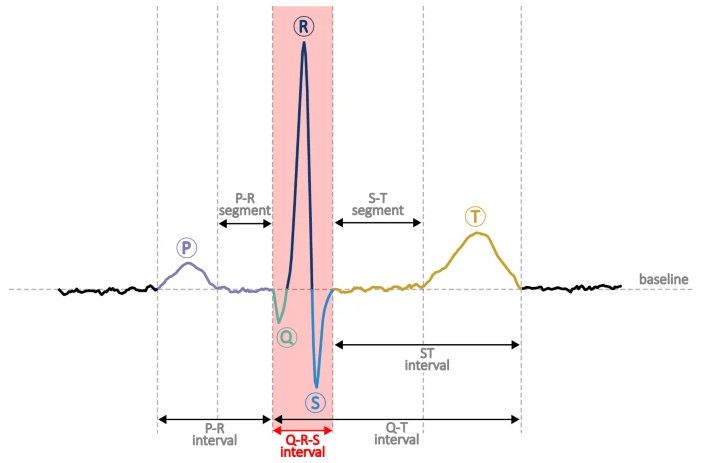
\includegraphics[width=0.7\textwidth]{esquema ECG.png}
    \caption{\ac{ecg} Schematic (Adapted from \cite{Dogan2023})}
    \label{fig:esquemaecg}
\end{figure}


\subsection{Related Works}

%The most popular signal that is used to describe pain is \ac{eda}, which measures skin conductivity, reflecting sweat gland activity, since it is related to the Sympathetic Nervous System \cite{Rojas2023}. - falar de SCL e GSR

In literature, the most common feature extracted from the \ac{ecg} is \ac{hrv}, which is related to time variations in R-R intervals. Nevertheless, other \ac{ecg} features have been analysed and selected as successful pain descriptors, along with features extracted from different physiological signals, like the \ac{emg} and \ac{eda}. For this signals' analysis, various machine learning models have been used, having achieved successful results throughout the years \cite{Moscato2022}\cite{Pais2025}.

For example, Pavlidou and Tsiknakis \cite{Pavlidou2025} used the BioVid Heat Pain dataset, in which heat pain was induced through a thermode, with the intent of obtaining significant features for pain classification. On that account, they extracted features from the \ac{ecg}, \ac{emg} and \ac{gsr} from 87 participants, where the first are HRV related. To detect pain, \acp{svm} and \ac{lstm} models were created while a \ac{loso} cross validation method was used to evaluate its intensity, distinguishing between a \ac{bl} and four levels of pain intensity (PA1, PA2, PA3 and PA4). The highest accuracy was obtained for multimodal approaches, with a maximum accuracy of 76.69\% for \ac{svm} and 77.21\% for \ac{lstm}. However, in unimodal approaches, \ac{gsr} features led to the best results, when compared with the other signals. Finally, the \ac{loso} method achieved a maximum accuracy of 82.83\% in \ac{bl} versus PA4, in accordance with the remaining results, where the best classification matched the models that compared the highest and lowest level of pain or the \ac{bl}.

Silva and Sebastião \cite{Silva2023} used a \ac{cpt} to induce pain in 36 participants, while eliciting distinct emotions through fear-inducing and neutral videos. This was done with the aim of measuring the effect of emotional contexts on physiological responses to pain. During the study, \ac{emg}, \ac{ecg}, \ac{eda}, and \ac{bp} data was collected. However, only the \ac{ecg} signals were analysed, using sliding windows for feature extraction. Subsequently, a variety of machine learning algorithms, including AdaBoost, Decision Trees, \ac{knn}, Linear Discriminant Analysis, Logistic Regression, \ac{rf}, and \acp{svm}, were employed across three classification strategies: dependent, session-independent, and participant-independent approaches. In the first, a maximum balanced accuracy of 97.4\% was obtained, while the second reached 97.7\% of balanced accuracy, which supports the hypothesis that the physiological response to pain remained consistent despite differing emotional contexts. Across the three approaches, the \ac{rf} and Adaboost models attained the best results. Meanwhile, the most relevant features were the amplitude of the S peaks, the amplitude of the T peaks, the amplitude of the T offset, and the amplitude of the R peaks (Ramplitude). Although emotion elicitation was intended, self-reported pain levels did not reveal statistically significant differences between the fear and neutral sessions. This result was attributed to patients being too focused on the pain to pay attention to the video.

Choosing an alternative approach, Balasubramani et al \cite{Balasubramani2025} analysed \ac{ecg} signals from 142 patients who underwent surgical procedures. Their methodology involved using two dimensional Continuous Wavelet Transform on the signals, and processing the results through a framework that combines a quantum neural network architecture and classical deep learning models. This new model achieved an accuracy of 94.8\% in pain assessment, implying that quantum transfer learning might acquire a fundamental role in future medical diagnostic systems. 






\chapter{References}



%\chapter{Results and Discussion}

\section{Identification of Significant Features}

This project employs unsupervised learning, specifically a K-means clustering algorithm, to identify the most relevant features for describing pain. This is done by generating clusters, where K is the number defined by the user for the quantity of centroids \cite{Ikotun2023}. The clustering technique partitions data according to specific distance metrics, and `cityblock' was chosen because of the way centroids are computed, that is, as the component-wise median of points in each cluster. Besides this, this metric measures the sum of absolute differences between data point coordinates, according to Equation \ref{eq:3} and assigns points to clusters based on this distance \cite{Ricken2023}.

\begin{equation} \label{eq:3}
d(x,y)=\sum_{i=1}^{n}\left| x_i-y_i \right|
\end{equation}

This clustering algorithm was applied to every possible pair of features, with the number of centroids set to $K=2$, using data from the second baseline and from the pain stimulation phase of the fifteen participants. It's important to mention that this analysis was firstly done with the first baseline but, comparing both options, the results were better using the second one, which may stem from the influence of the emotional stimuli in the pain felt by the participants.

The result of clustering applied to two features -- the medians of the median of the S peak amplitude (x-axis) and of the median of the R offset amplitude (y-axis) -- is displayed in Figure \ref{fig:cluster} (right). In it, the two clusters defined by the algorithm can be seen, as well as X's in the position of the clusters' centroids.
For comparison, scattering graphics were plotted for each two features, as can be seen in Figure \ref{fig:cluster} (left). The incorrect matches made by the clustering algorithm are circled in black.

\begin{figure}[h!]
    \centering
    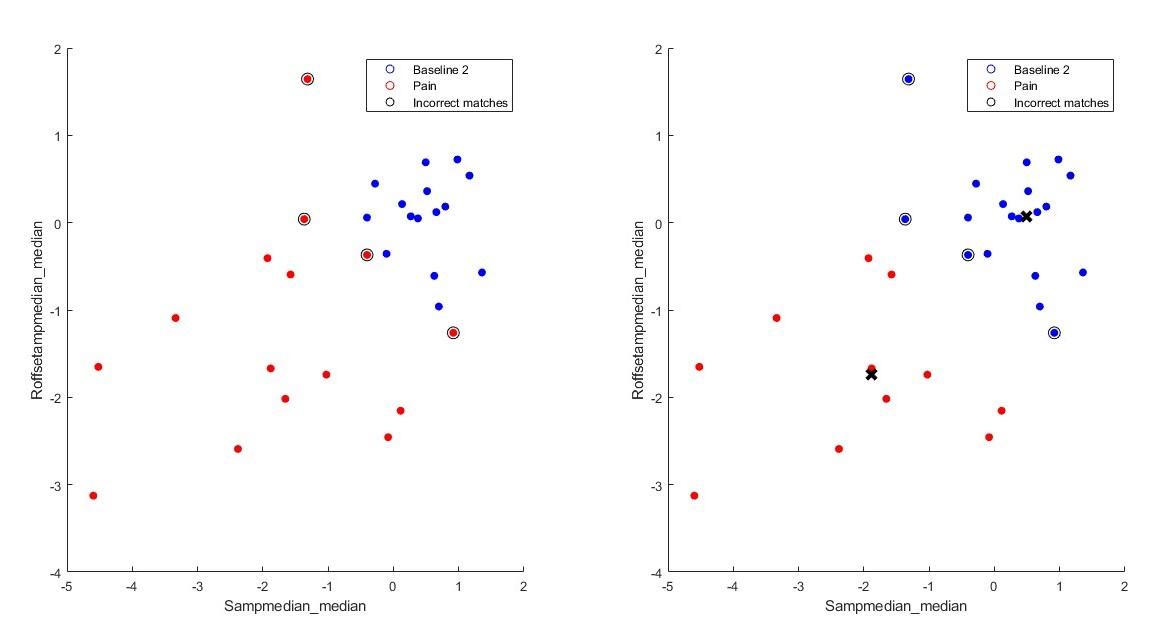
\includegraphics[width=1.0\textwidth]{cluster.jpg}
    \caption{Scattering plot with data from baseline 2 and pain (left), and with the result of K-means clustering (right), when comparing the Roffsetampmedian\_median and Sampmedian\_median.}
    \label{fig:cluster}
\end{figure}

\pagebreak
Only the pairs of features where more than 80\% of the observations were correctly predicted were considered valid. A network map illustrating these pairs was plotted in Figure \ref{fig:map80}. In this map, each circle corresponds to a feature, while the lines connecting them showcase the combinations that met the accuracy threshold. Additionally, the size of the circles is proportional to how many times that specific feature, paired with another, contributed to successful clustering. These results suggest that these five features, Roffsetampmedian\_median, Sampmedian\_median, Entropydb4Approx\_median, and Entropydb9Approx\_median, when paired with each other, are the most effective in distinguishing pain from no pain. \hl{A possible takeaway from this result is that pain affects the intensity of ventricular polarization, since the S wave and R offset are related to it. Regarding the entropy, pain affects it the most in the low frequencies of the \ac{ecg} signal, for both the db4 and db9 wavelets. This might entail that the QRS complex, as concluded before, and the fluctuations of the signal also affect pain.}





\begin{figure}[h!]
    \centering
    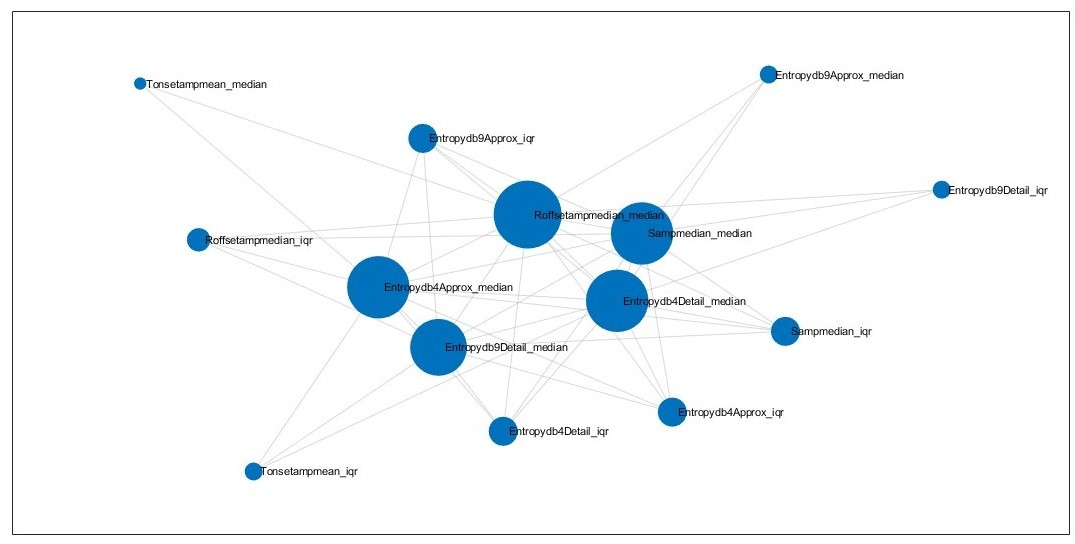
\includegraphics[width=1.0\textwidth]{map80.jpg}
    \caption{Network diagram of the pairs of features with more than 80\% correctly predicted observations.}
    \label{fig:map80}
\end{figure}



\subsection{Multiple Comparison Test}

To determine whether these features can distinguish pain from the lack of it in spite of the context, statistical analysis was performed through a multiple comparison test applied to both the baselines and to the pain phase. This was done for each participant first, using the original features that resulted in the selected ones, and then for the extracted features. Firstly, a one-way \ac{anova} was applied to the three groups. This test evaluates whether there are statistically significant differences between the means of each group. Afterwards, the Tukey-Kramer method, also known as the \ac{hsd} method, was performed as a post-hoc test to determine whether the differences detected by the \ac{anova} test are significant. This is done by taking the absolute value of the difference between pairs of means and dividing it by the standard error of the mean \cite{Nanda2021}. %The SE is in turn the square root of (variance divided by sample size)


Analysing each participant's data individually, regarding the median of the R offset amplitude, the means of the pain and baseline phases were different for 100\% of the participants, with 20\% of the baselines' means being coincident. For the median of the S amplitude, there was 93\% of successful pain and baselines' means distinction, where 43\% corresponded to similar means when comparing the baselines.
Lastly, the entropy of the approximation of the db4 and db9 wavelets acquired analogous results, with 80\% of the participants' pain and baselines' means being significantly different. 25\% of these participants' baselines 1 and 2 had similar means for both of these features. These results suggest that, for most participants, these features are successful in describing pain. Additionally, it's viable that the video watched by each participant has affected not only the entropy of the \ac{ecg} and the R offset, but mostly the amplitude of the S wave. In Figures \ref{fig:multcompR} to \ref{fig:multcomp9}, examples of this multiple comparison tests are displayed for each feature. 



\begin{figure}[htbp]
    \centering
    \begin{minipage}{0.49\textwidth}
        \centering
        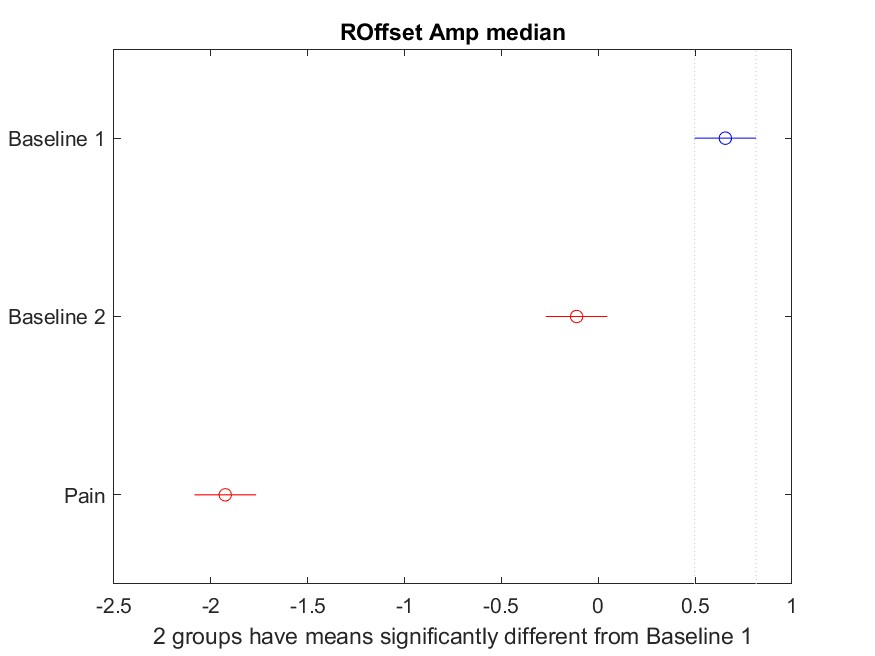
\includegraphics[width=6.8cm]{ROffset Amp median_part2.jpg}
        \caption{Multiple comparison test of the R offset amplitude for a participant's baselines and pain phase.}
        \label{fig:multcompR}
    \end{minipage}
    \hfill
    \begin{minipage}{0.49\textwidth}
        \centering
        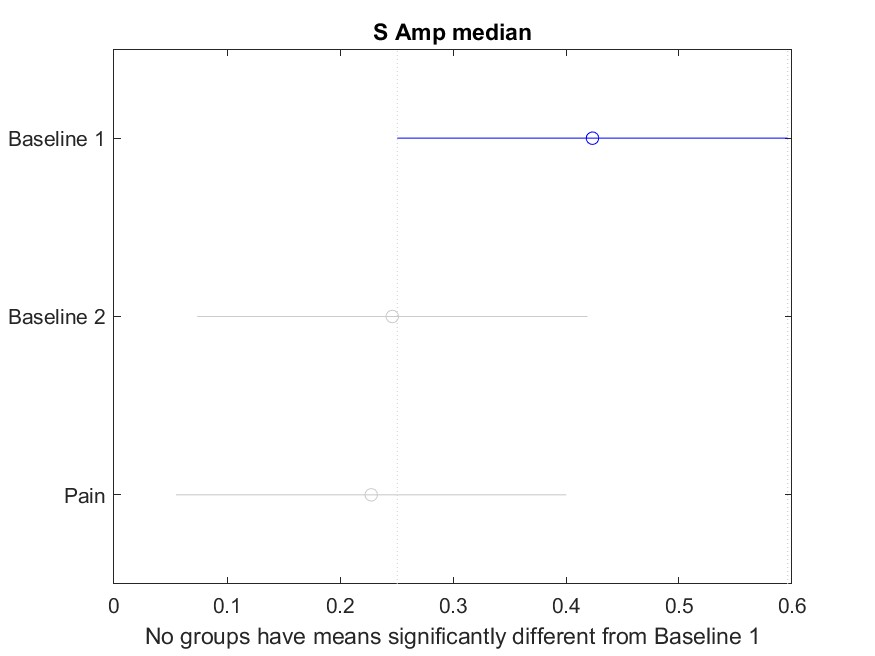
\includegraphics[width=6.8cm]{S Amp median_part2.jpg}
        \caption{Multiple comparison test of the S wave amplitude for a participant's baselines and pain phase.}
        \label{fig:multcompS}
    \end{minipage}
\end{figure}



\begin{figure}[htbp]
    \centering
    \begin{minipage}{0.49\textwidth}
        \centering
        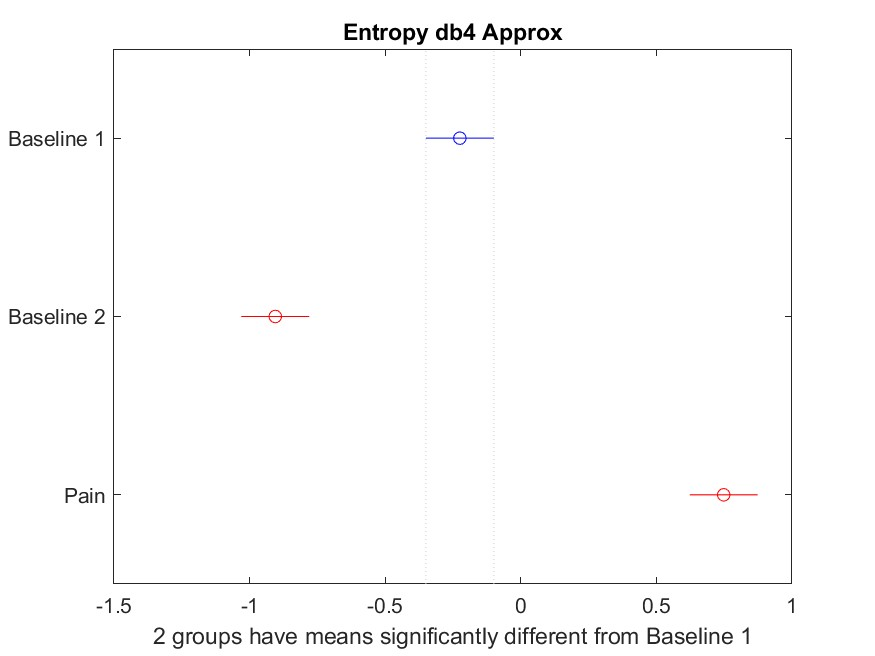
\includegraphics[width=6.8cm]{Entropy db4 Approx_part2.jpg}
        \caption{Multiple comparison test of the entropy of the db4 approximation for a participant's baselines and pain phase.}
        \label{fig:multcomp4}
    \end{minipage}
    \hfill
    \begin{minipage}{0.49\textwidth}
        \centering
        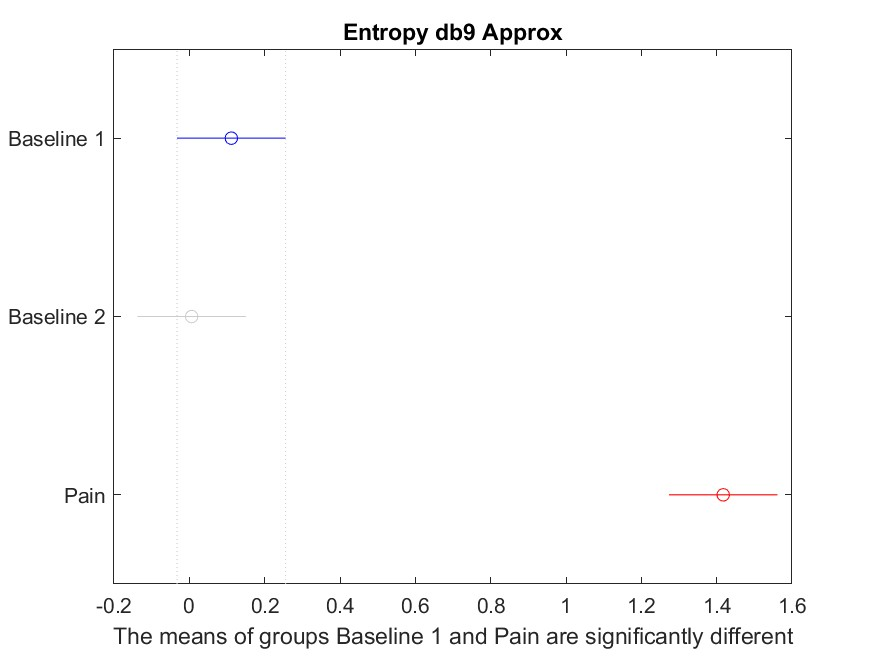
\includegraphics[width=6.8cm]{Entropy db9 Approx_part34.jpg}
        \caption{Multiple comparison test of the entropy of the db9 approximation for a participant's baselines and pain phase.}
        \label{fig:multcomp9}
    \end{minipage}
\end{figure}

\pagebreak

On the other hand, the result of this test for the selected extracted features is portrayed in Figure \ref{fig:five_images}. As can be seen, the baselines' means are significantly different from the pain phase's for all the selected features, which supports the idea that pain has an impact on both the S wave and entropy. 
Furthermore, the means of the baselines are similar in all the graphics, which means both can be used to describe pain. However, there’s a slight difference between the baselines for the amplitude of the S wave. This might be due to the visual stimulus having an impact on the ventricular polarization.




\begin{figure}[htbp]
    \centering
    % First row of 2 images
    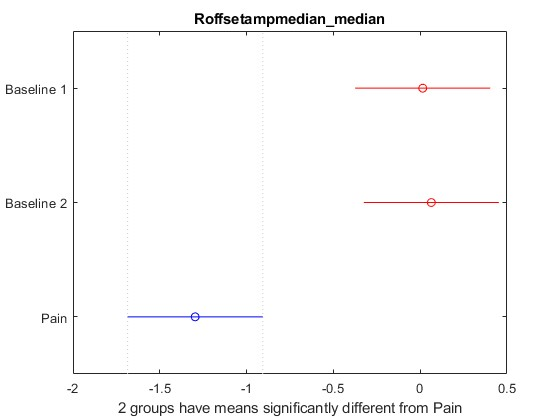
\includegraphics[width=0.49\linewidth]{multcompareR.jpg}
    \hfill
    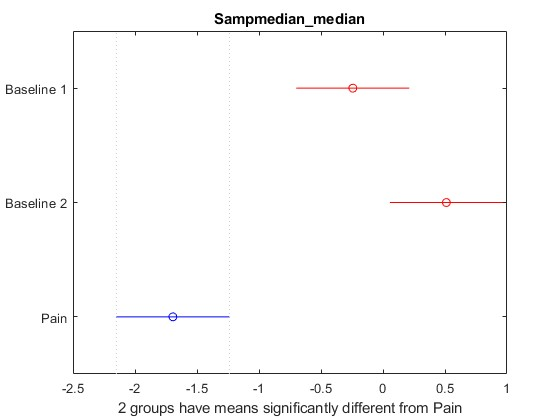
\includegraphics[width=0.49\linewidth]{multcompareS.jpg}
    \vspace{0.5em}  % space between rows
    % Second row of 2 images
    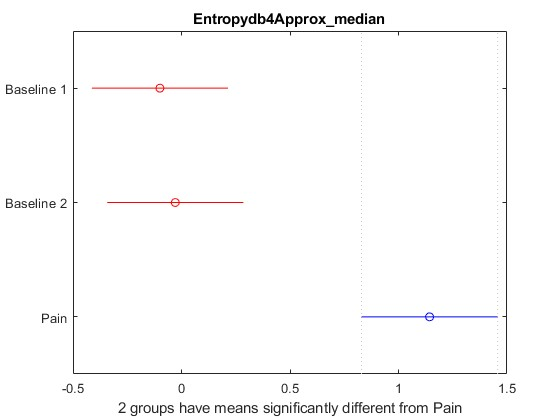
\includegraphics[width=0.49\linewidth]{multcompare4approx.jpg}
    \hfill
    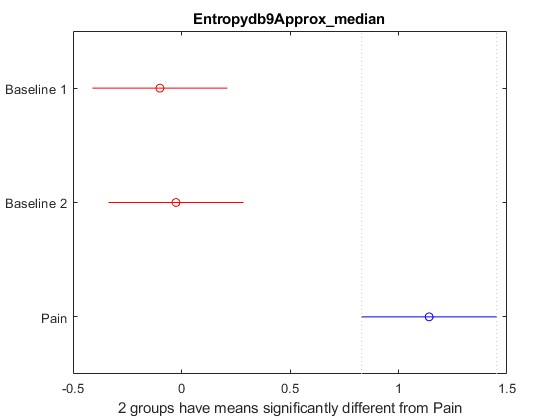
\includegraphics[width=0.49\linewidth]{multcompare9approx.jpg}
    \vspace{0.5em}  % space between rows
    \caption{Multiple comparison test (\ac{anova} + HSD) applied to both the baselines and to the pain phase, for each of the selected features.}
    \label{fig:five_images}
\end{figure}

\pagebreak 
\section{K-Nearest Neighbours}

In order to validate the results of this project, a Classification Learner algorithm, particularly, a \ac{knn} classifier was employed on the selected features. This classifier is widely used due to its simplicity and effectiveness but, for this project, it was chosen because of its classification technique's similarity to the clustering algorithm. \ac{knn} classification starts with the determination of the K-nearest neighbours, which is done by computing the distance between an unknown example $q$, that must be classified, and $x_i$ training samples. This distance is described by Equation \ref{eq:4}, which is a summation for all the features in $F$, with $w_f$ being the weight for each feature and $\delta$ a specific distance metric \cite{Cunningham2022}. Then, a majority voting is applied and $q$ is characterised as the class of the majority of its K-nearest neighbours \cite{Papanikolaou2021}.

\begin{equation} \label{eq:4}
d(q,x_i)=\sum_{f\epsilon F}^{}w_f\delta(q_f,x_{if})
\end{equation}



To create this classifier, MATLAB's Classification Learner app was used, along with the processed features from the aforementioned fifteen participants. For the distance metric, Euclidian distance was chosen. This metric is computed as the square root of the sum of squared differences between the elements of both vectors, according to Equation \ref{eq:4}.

\begin{equation} \label{eq:4}
\delta(x,y)=\sqrt{\sum_{i=1}^{n}(x_i-y_i)^2}
\end{equation}

The remaining hyperparameters were selected using Bayesian optimisation. The goal of this optimisation is to find the ideal combination of parameters that minimizes cross-validation loss. After performing a search with 30 iterations, the optimised parameters were selected and used in the model. These are portrayed in Table \ref{table:hyperparameters}. 

\begin{table}[h]
    \centering
    \captionsetup{justification=raggedright, singlelinecheck=false}
    \caption{Hyperparameters optimisation search range and results.}
    \renewcommand{\arraystretch}{1.2}

    \begingroup
    \hyphenpenalty=10000
    \exhyphenpenalty=10000
    \sloppy
    \begin{tabular}{@{}>{\RaggedRight\arraybackslash}p{4.3cm} >{\RaggedRight\arraybackslash}p{5.7cm} >{\RaggedRight\arraybackslash}p{4cm}@{}}
        \hline
        \textbf{Hyperparameters} & \textbf{Search Range} & \textbf{Optimised Values} \\
        \midrule
        Number of neighbours & 1-15 & 2 \\
        [1ex]
        Distance weight & Equal, Inverse, Squared inverse & Equal \\
        [1ex]
        Standardised & True, False & False \\
    \end{tabular}
    \endgroup
    \label{table:hyperparameters}
\end{table}    



Once the hyperparameters were selected, the model was trained using the fifteen participants' features as the training set. This was done through fivefold cross-validation, that uses one fifth of the data to evaluate the model in each iteration. Once the \ac{knn} model was complete, the processing pipeline was applied to the remaining 36 participants' data to create a training dataset. Then, the model was applied to this set, predicting whether a value had derived from the baseline or pain stimulation phase. To compare these predictions with the true values, a confusion matrix was plotted in Figure \ref{fig:confusiontest}. This allows for the computation of the following variables:

\begin{itemize}
   \item \textbf{\ac{tp}:} pain observations correctly predicted.
   \item \textbf{\ac{fp}:} pain observations incorrectly predicted.
   \item \textbf{\ac{tn}:} baseline observations correctly predicted.
   \item \textbf{\ac{fn}:} baseline observations incorrectly predicted.
 \end{itemize}

 \begin{figure}[h!]
    \centering
    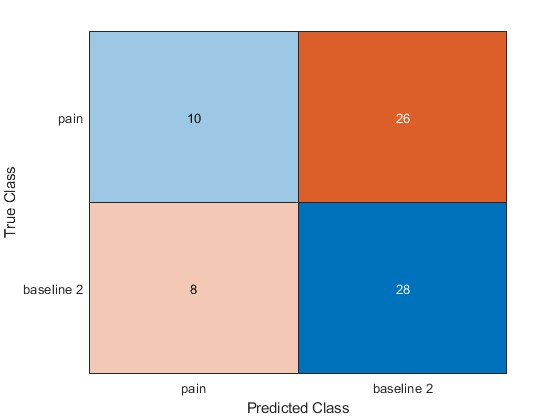
\includegraphics[width=0.7\textwidth]{confusion test.jpg}
    \caption{Confusion matrix for KNN model testing.}
    \label{fig:confusiontest}
\end{figure}

These variables can be used to calculate metrics for classification models' evaluation, such as sensitivity, precision, accuracy, and F-score. Sensitivity, also known as True Positive Rate, is obtained by dividing the number of \ac{tp} for the sum of \ac{tp} and \ac{fn}. On the other hand, specificity, or True Negative Rate, corresponds to the number of \ac{tn} divided by the sum of \ac{tn} and \ac{fp}. Meanwhile, precision is computed as the ratio between the \ac{tp} and the total number of pain predictions, while accuracy is computed as the sum of \ac{tp} and \ac{tn} divided by the total number of observations \cite{Vujovic2021}. 

\pagebreak

\begin{table}[h]
    \centering
    \captionsetup{justification=raggedright, singlelinecheck=false}
    \caption{Features for pain classification after data preparation procedures.}
    \renewcommand{\arraystretch}{1.2}

    \begingroup
    \hyphenpenalty=10000
    \exhyphenpenalty=10000
    \sloppy
    \begin{tabular}{@{}>{\RaggedRight\arraybackslash}p{4.5cm} >{\RaggedRight\arraybackslash}p{3.5cm}@{}}
        \hline
        \textbf{Evaluation Metric} & \textbf{Percentage} \\
        \midrule
        Sensitivity & 27.8\% \\
        [1ex]
        Specificity & 77.8\% \\
        [1ex]
        Precision & 55.6\% \\
        [1ex]
        Accuracy & 52.8\% \\
    \end{tabular}
    \endgroup
    \label{table:evaluationmetrics}
\end{table}

As shown in Table \ref{table:evaluationmetrics}, the \ac{knn} model achieved a low sensitivity of 27.8\%. This implies that the model was unsuccessful in correctly identifying true cases of pain, contesting the validity of these features for pain description. In contrast, the specificity was relatively high at 77.8\%, indicating that the model was more effective in correctly identifying the absence of pain. Additionally, an accuracy of 52.8\% was obtained, which indicates that approximately half of the predictions made on the test set were correct. Meanwhile, precision reached 55.6\%, suggesting that slightly more than half of the observations classified as pain were true positives. 

%%%%%%%%%%%%%%%%%%%%%%%%%%%%%%%%%%%%%%%%%%%%%%%%%%%%%%%
% End of Thesis text 
%%%%%%%%%%%%%%%%%%%%%%%%%%%%%%%%%%%%%%%%%%%%%%%%%%%%%%%

\backmatter

%%%%%%%%%%%%%%%%%%%%%%%%%%%%%%%%%%%%%%%%%%%%%%%%%%%%%%%
% Print all used references
%%%%%%%%%%%%%%%%%%%%%%%%%%%%%%%%%%%%%%%%%%%%%%%%%%%%%%%

\begingroup
\renewcommand{\bibfont}{\footnotesize}
% Redefine References name to Portuguese
% Change if you are using english
\defbibheading{bibliography}[References]{
	\chapter{#1}
}
\SingleSpacing
\setlength\bibitemsep{8pt}
\printbibliography[heading=bibliography]
\endgroup


%%%%%%%%%%%%%%%%%%%%%%%%%%%%%%%%%%%%%%%%%%%%%%%%%%%%%%%
% Load appendix
%%%%%%%%%%%%%%%%%%%%%%%%%%%%%%%%%%%%%%%%%%%%%%%%%%%%%%%

\mainmatterWithoutReset
\appendix

\include{chapters/appendix-more}

\end{document}